\documentclass[tikz,border=20pt]{standalone}
\usepackage{tikz}
\usetikzlibrary{arrows.meta, positioning, calc}
\usepackage{amsmath,amssymb}

\begin{document}
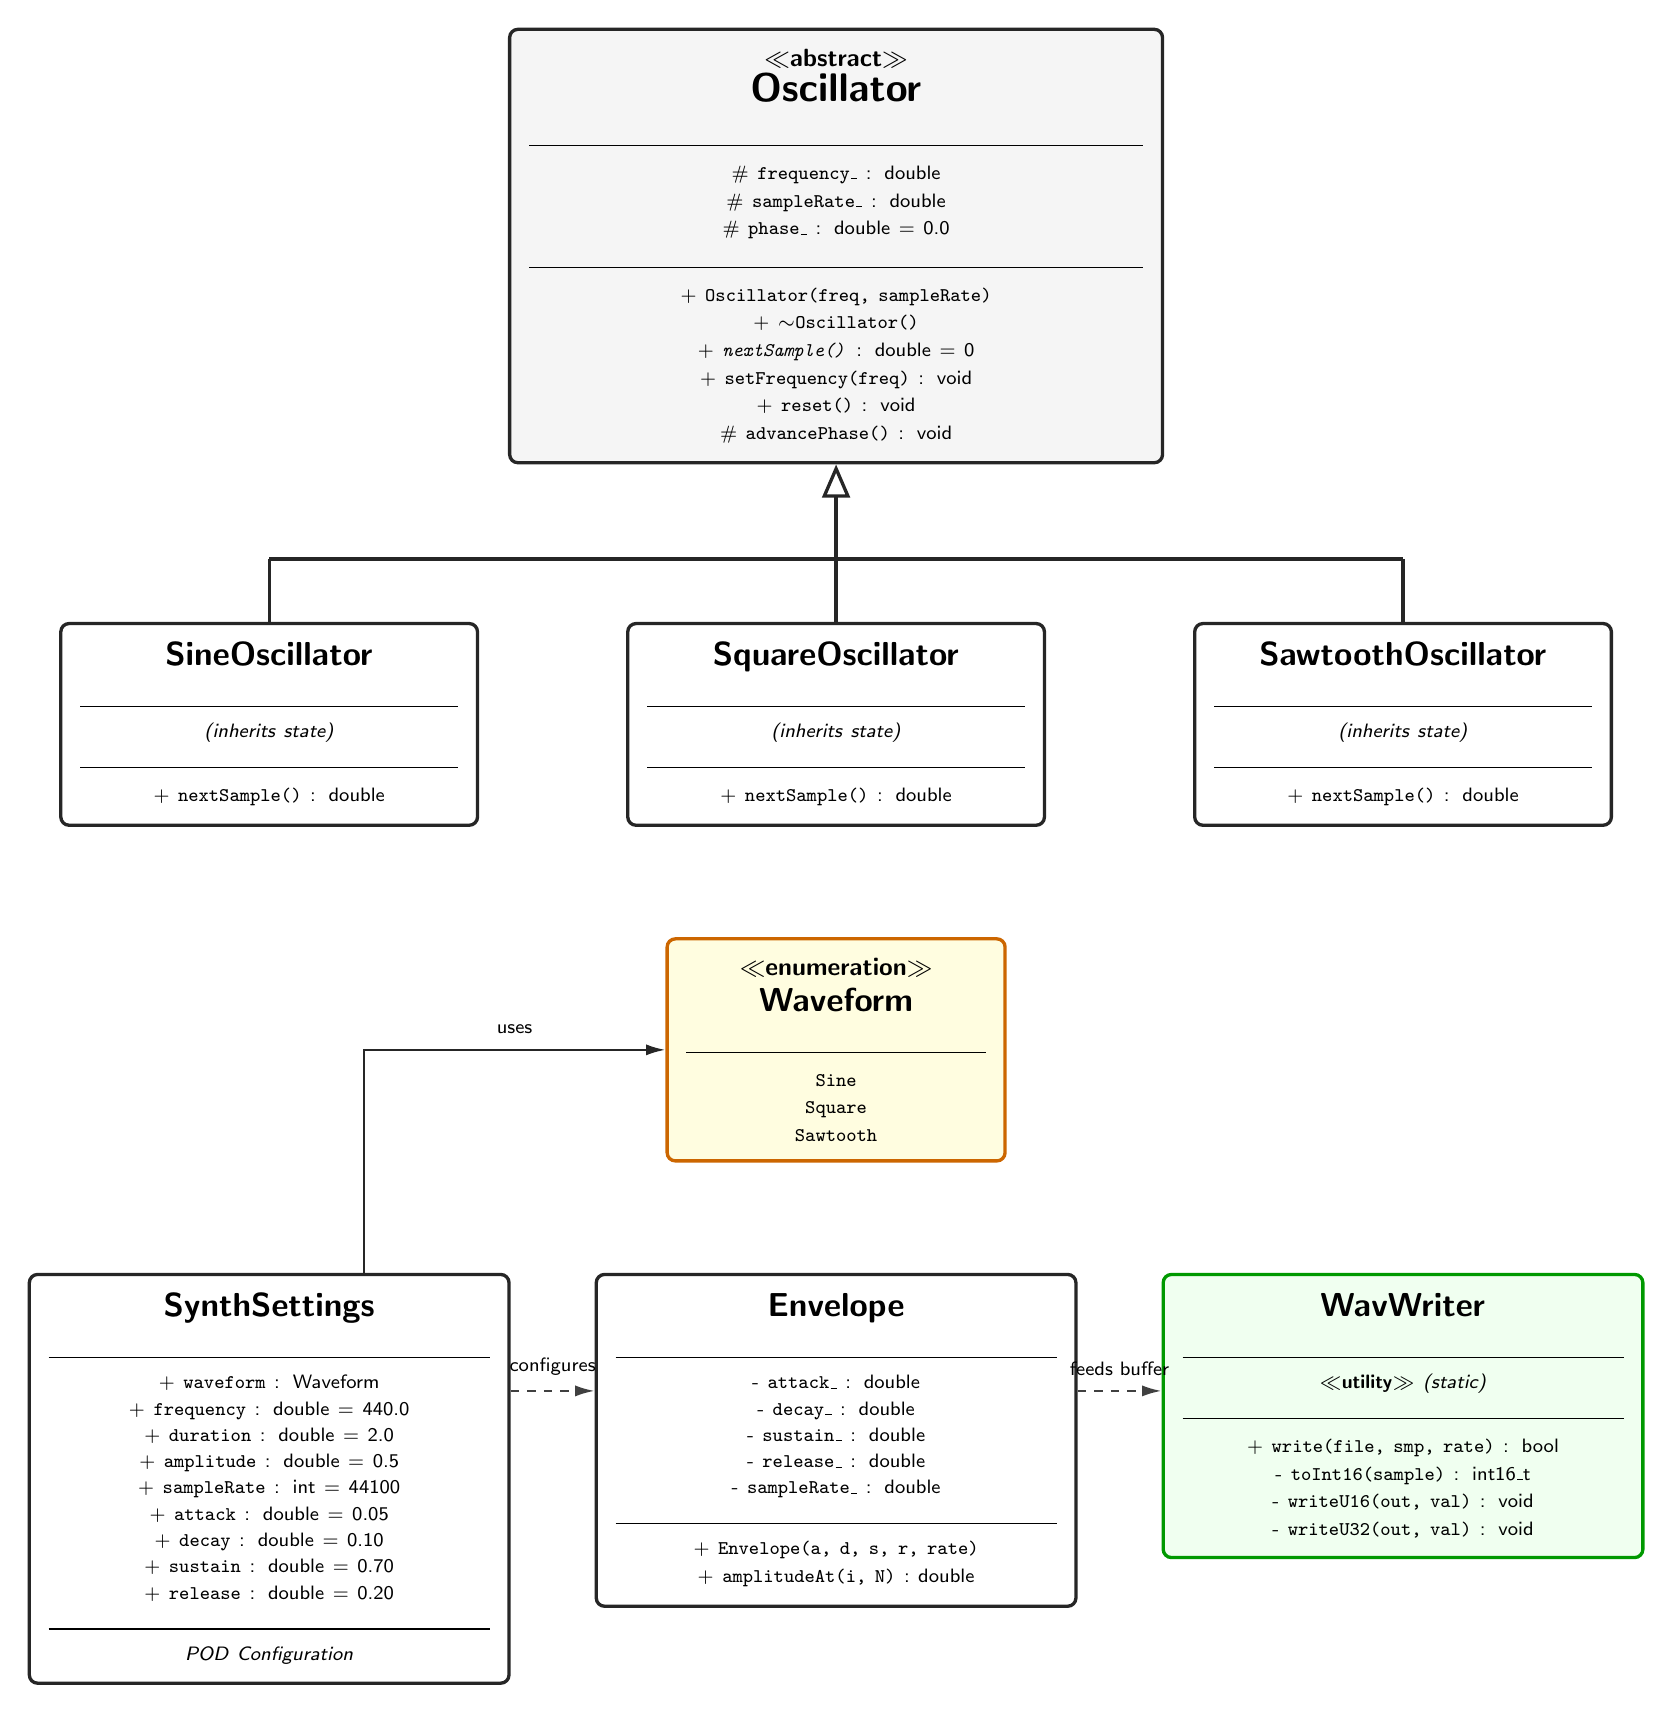
\begin{tikzpicture}[
    font=\small\sffamily,
    umlClass/.style={
        draw=black!85,
        very thick,
        fill=white,
        rounded corners=3pt,
        inner sep=7pt,
        align=left
    },
    umlAbstract/.style={
        umlClass,
        fill=gray!8
    },
    umlEnum/.style={
        umlClass,
        fill=yellow!12,
        draw=orange!80!black
    },
    umlWriter/.style={
        umlClass,
        fill=green!6,
        draw=green!60!black
    },
    depend/.style={
        -{Latex[length=7pt, width=4pt]},
        dashed,
        thick,
        draw=black!75
    },
    assoc/.style={
        -{Latex[length=7pt, width=4pt]},
        thick,
        draw=black!85
    }
]

    % =========================================================================
    % 1. TOP ROW: Abstract Base Class (Oscillator)
    % =========================================================================
    \node[umlAbstract, text width=7.8cm, anchor=north] (oscillator) at (0, 0) {
        \centering $\ll$\textbf{abstract}$\gg$\\[2pt]
        \centering\textbf{\Large Oscillator}\\[5pt]
        \rule{\linewidth}{0.5pt}\\[4pt]
        \scriptsize
        \# \texttt{frequency\_} : double\\[2pt]
        \# \texttt{sampleRate\_} : double\\[2pt]
        \# \texttt{phase\_} : double = 0.0\\[4pt]
        \rule{\linewidth}{0.5pt}\\[4pt]
        \scriptsize
        + \texttt{Oscillator(freq, sampleRate)}\\[2pt]
        + \texttt{$\sim$Oscillator()}\\[2pt]
        + \texttt{\textit{nextSample()}} : double = 0\\[2pt]
        + \texttt{setFrequency(freq)} : void\\[2pt]
        + \texttt{reset()} : void\\[2pt]
        \# \texttt{advancePhase()} : void\\[2pt]
    };

    % =========================================================================
    % 2. INHERITANCE BUS BAR (Guaranteed 1.2 cm below Oscillator bottom)
    % =========================================================================
    \coordinate (bus) at ([yshift=-1.2cm]oscillator.south);
    \coordinate (stemLeft) at (-7.2, 0 |- bus);
    \coordinate (stemCenter) at (bus);
    \coordinate (stemRight) at (7.2, 0 |- bus);

    % Upward arrow to Oscillator bottom with open UML triangle
    \draw[very thick, draw=black!85, -{Triangle[open, length=12pt, width=10pt]}] (stemCenter) -- (oscillator.south);

    % Horizontal distribution bus bar
    \draw[very thick, draw=black!85] (stemLeft) -- (stemRight);

    % =========================================================================
    % 3. SECOND ROW: Concrete Waveform Oscillators (0.8 cm below bus bar)
    % =========================================================================
    \node[umlClass, text width=4.8cm, anchor=north] (sineOsc) at ([yshift=-0.8cm]stemLeft) {
        \centering\textbf{\large SineOscillator}\\[4pt]
        \rule{\linewidth}{0.5pt}\\[3pt]
        \centering\scriptsize\textit{(inherits state)}\\[3pt]
        \rule{\linewidth}{0.5pt}\\[4pt]
        \centering\scriptsize + \texttt{nextSample()} : double\\[2pt]
    };

    \node[umlClass, text width=4.8cm, anchor=north] (squareOsc) at ([yshift=-0.8cm]stemCenter) {
        \centering\textbf{\large SquareOscillator}\\[4pt]
        \rule{\linewidth}{0.5pt}\\[3pt]
        \centering\scriptsize\textit{(inherits state)}\\[3pt]
        \rule{\linewidth}{0.5pt}\\[4pt]
        \centering\scriptsize + \texttt{nextSample()} : double\\[2pt]
    };

    \node[umlClass, text width=4.8cm, anchor=north] (sawOsc) at ([yshift=-0.8cm]stemRight) {
        \centering\textbf{\large SawtoothOscillator}\\[4pt]
        \rule{\linewidth}{0.5pt}\\[3pt]
        \centering\scriptsize\textit{(inherits state)}\\[3pt]
        \rule{\linewidth}{0.5pt}\\[4pt]
        \centering\scriptsize + \texttt{nextSample()} : double\\[2pt]
    };

    % Drop stems connecting bus bar to derived oscillators
    \draw[very thick, draw=black!85] (stemLeft) -- (sineOsc.north);
    \draw[very thick, draw=black!85] (stemCenter) -- (squareOsc.north);
    \draw[very thick, draw=black!85] (stemRight) -- (sawOsc.north);

    % =========================================================================
    % 4. THIRD ROW: Waveform Enumeration (1.4 cm below SquareOscillator)
    % =========================================================================
    \node[umlEnum, text width=3.8cm, anchor=north] (waveformEnum) at ([yshift=-1.4cm]squareOsc.south) {
        \centering $\ll$\textbf{enumeration}$\gg$\\[2pt]
        \centering\textbf{\large Waveform}\\[4pt]
        \rule{\linewidth}{0.5pt}\\[4pt]
        \centering\scriptsize
        \texttt{Sine}\\[2pt]
        \texttt{Square}\\[2pt]
        \texttt{Sawtooth}\\[2pt]
    };

    % =========================================================================
    % 5. FOURTH ROW: SynthSettings, Envelope, and WavWriter
    % =========================================================================
    \node[umlClass, text width=5.6cm, anchor=north] (envelope) at ([yshift=-1.4cm]waveformEnum.south) {
        \centering\textbf{\large Envelope}\\[4pt]
        \rule{\linewidth}{0.5pt}\\[3pt]
        \scriptsize
        - \texttt{attack\_} : double\\[1.5pt]
        - \texttt{decay\_} : double\\[1.5pt]
        - \texttt{sustain\_} : double\\[1.5pt]
        - \texttt{release\_} : double\\[1.5pt]
        - \texttt{sampleRate\_} : double\\[3pt]
        \rule{\linewidth}{0.5pt}\\[3pt]
        \scriptsize
        + \texttt{Envelope(a, d, s, r, rate)}\\[2pt]
        + \texttt{amplitudeAt(i, N)} : double\\[2pt]
    };

    \node[umlClass, text width=5.6cm, anchor=north] (settings) at (envelope.north -| stemLeft) {
        \centering\textbf{\large SynthSettings}\\[4pt]
        \rule{\linewidth}{0.5pt}\\[3pt]
        \scriptsize
        + \texttt{waveform} : Waveform\\[1.5pt]
        + \texttt{frequency} : double = 440.0\\[1.5pt]
        + \texttt{duration} : double = 2.0\\[1.5pt]
        + \texttt{amplitude} : double = 0.5\\[1.5pt]
        + \texttt{sampleRate} : int = 44100\\[1.5pt]
        + \texttt{attack} : double = 0.05\\[1.5pt]
        + \texttt{decay} : double = 0.10\\[1.5pt]
        + \texttt{sustain} : double = 0.70\\[1.5pt]
        + \texttt{release} : double = 0.20\\[3pt]
        \rule{\linewidth}{0.5pt}\\[3pt]
        \centering\scriptsize\textit{POD Configuration}\\[2pt]
    };

    \node[umlWriter, text width=5.6cm, anchor=north] (wavWriter) at (envelope.north -| stemRight) {
        \centering\textbf{\large WavWriter}\\[4pt]
        \rule{\linewidth}{0.5pt}\\[3pt]
        \centering\scriptsize $\ll$\textbf{utility}$\gg$ \textit{(static)}\\[3pt]
        \rule{\linewidth}{0.5pt}\\[4pt]
        \scriptsize
        + \texttt{write(file, smp, rate)} : bool\\[2pt]
        - \texttt{toInt16(sample)} : int16\_t\\[2pt]
        - \texttt{writeU16(out, val)} : void\\[2pt]
        - \texttt{writeU32(out, val)} : void\\[2pt]
    };

    % =========================================================================
    % 6. ASSOCIATIONS & DEPENDENCIES (Zero overlaps, clean routes)
    % =========================================================================
    % SynthSettings uses Waveform: orthogonal path up from settings.north then right to waveformEnum.west
    \draw[assoc] ([xshift=1.2cm]settings.north) |- node[near end, above=2pt, font=\scriptsize\sffamily] {uses} (waveformEnum.west);

    % SynthSettings configures Envelope: straight horizontal dashed arrow across generous gap
    \draw[depend] ([yshift=-1.5cm]settings.north east) -- node[midway, above=2pt, font=\scriptsize\sffamily] {configures} ([yshift=-1.5cm]envelope.north west);

    % Envelope feeds buffer to WavWriter: straight horizontal dashed arrow across generous gap
    \draw[depend] ([yshift=-1.5cm]envelope.north east) -- node[midway, above=2pt, font=\scriptsize\sffamily] {feeds buffer} ([yshift=-1.5cm]wavWriter.north west);

\end{tikzpicture}
\end{document}
